\chapter{Implémentation du M1}
Dans ce chapitre nous définirons une application \textit{Client-Serveur} en implémentant le méta-model proposé au chapitre \ref{chap:M2}.

\section{Démarche modélisation M1}
L'énoncé du projet/TP nous propose un serveur avec les fonctionnalités suivantes :

\begin{itemize}
\item \verb+ConnexionManager+ :   Gestion des connexions. 
\item  \verb+Database+ :  Gestion de la base de données.
\item \verb+SecurityManager+ :  Gestion d'un système de sécurité.
\end{itemize}

Un composant étant par définition la spécification d'une fonctionnalités, chacune des fonctionnalités précedement listées est un \verb+Composant+. Chaque service de chaque composant a son port requis relié au rôle fournis  du connecteur ( et inversement pour les ports fournis et rôles requis).

Les liaisons est ces différents composant et le client sont explicitées dans la figure \ref{fig:desSer}.
\begin{figure}[htb]
  \centering
  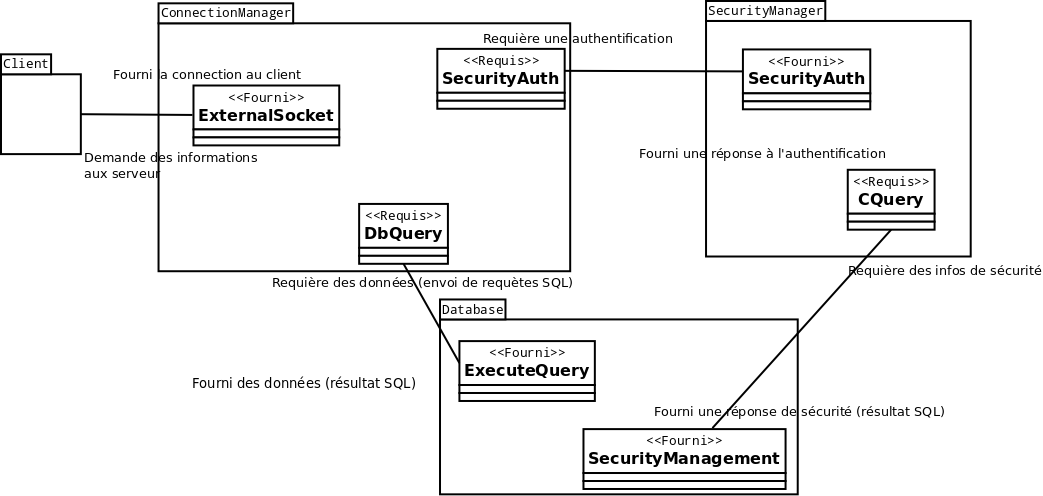
\includegraphics[scale=0.32]{img/DescribServeur}
  \caption{Description du Serveur}
  \label{fig:desSer}.
\end{figure}


\subsection{ConnexionManager}
Ce composant possède les services suivants : 
\begin{itemize}
\item 
  \verb+ServiceFExternalSocket+ : Fournit une connexion au serveur.
\item 
  \verb+ServicerDDBQuery+ :  requière une réponse de la base de données (requête SQL).
\item 
  \verb+ServiceRSecurityManager+ :  requière une validation de l'authentification
\end{itemize}


\subsection{Database}
Ce composant possède les services suivants : 
\begin{itemize}
\item 
  \verb+ServiceFSecurityManagement+ :  fournit une réponse à la requête de sécurité.
\item 
  \verb+ServicerFExecuteSQL+ :  fournit une réponse à une requête du client (par le ConnexionManager).
\end{itemize}

\subsection{SecurityManager}
Ce composant possède les services suivants : 
\begin{itemize}
\item 
  \verb+ServiceFSecurityAuth+ : fournit une validation de la demande de connexion.
\item 
  \verb+ServicerSecurityManager+ :  requière une réponde de sécurité de la base de données (requête SQL).
\end{itemize}

\section{Diagramme M1}
\pagestyle{empty}
%\newgeometry{a3paper}
\begin{figure}[htb]
  \centering
  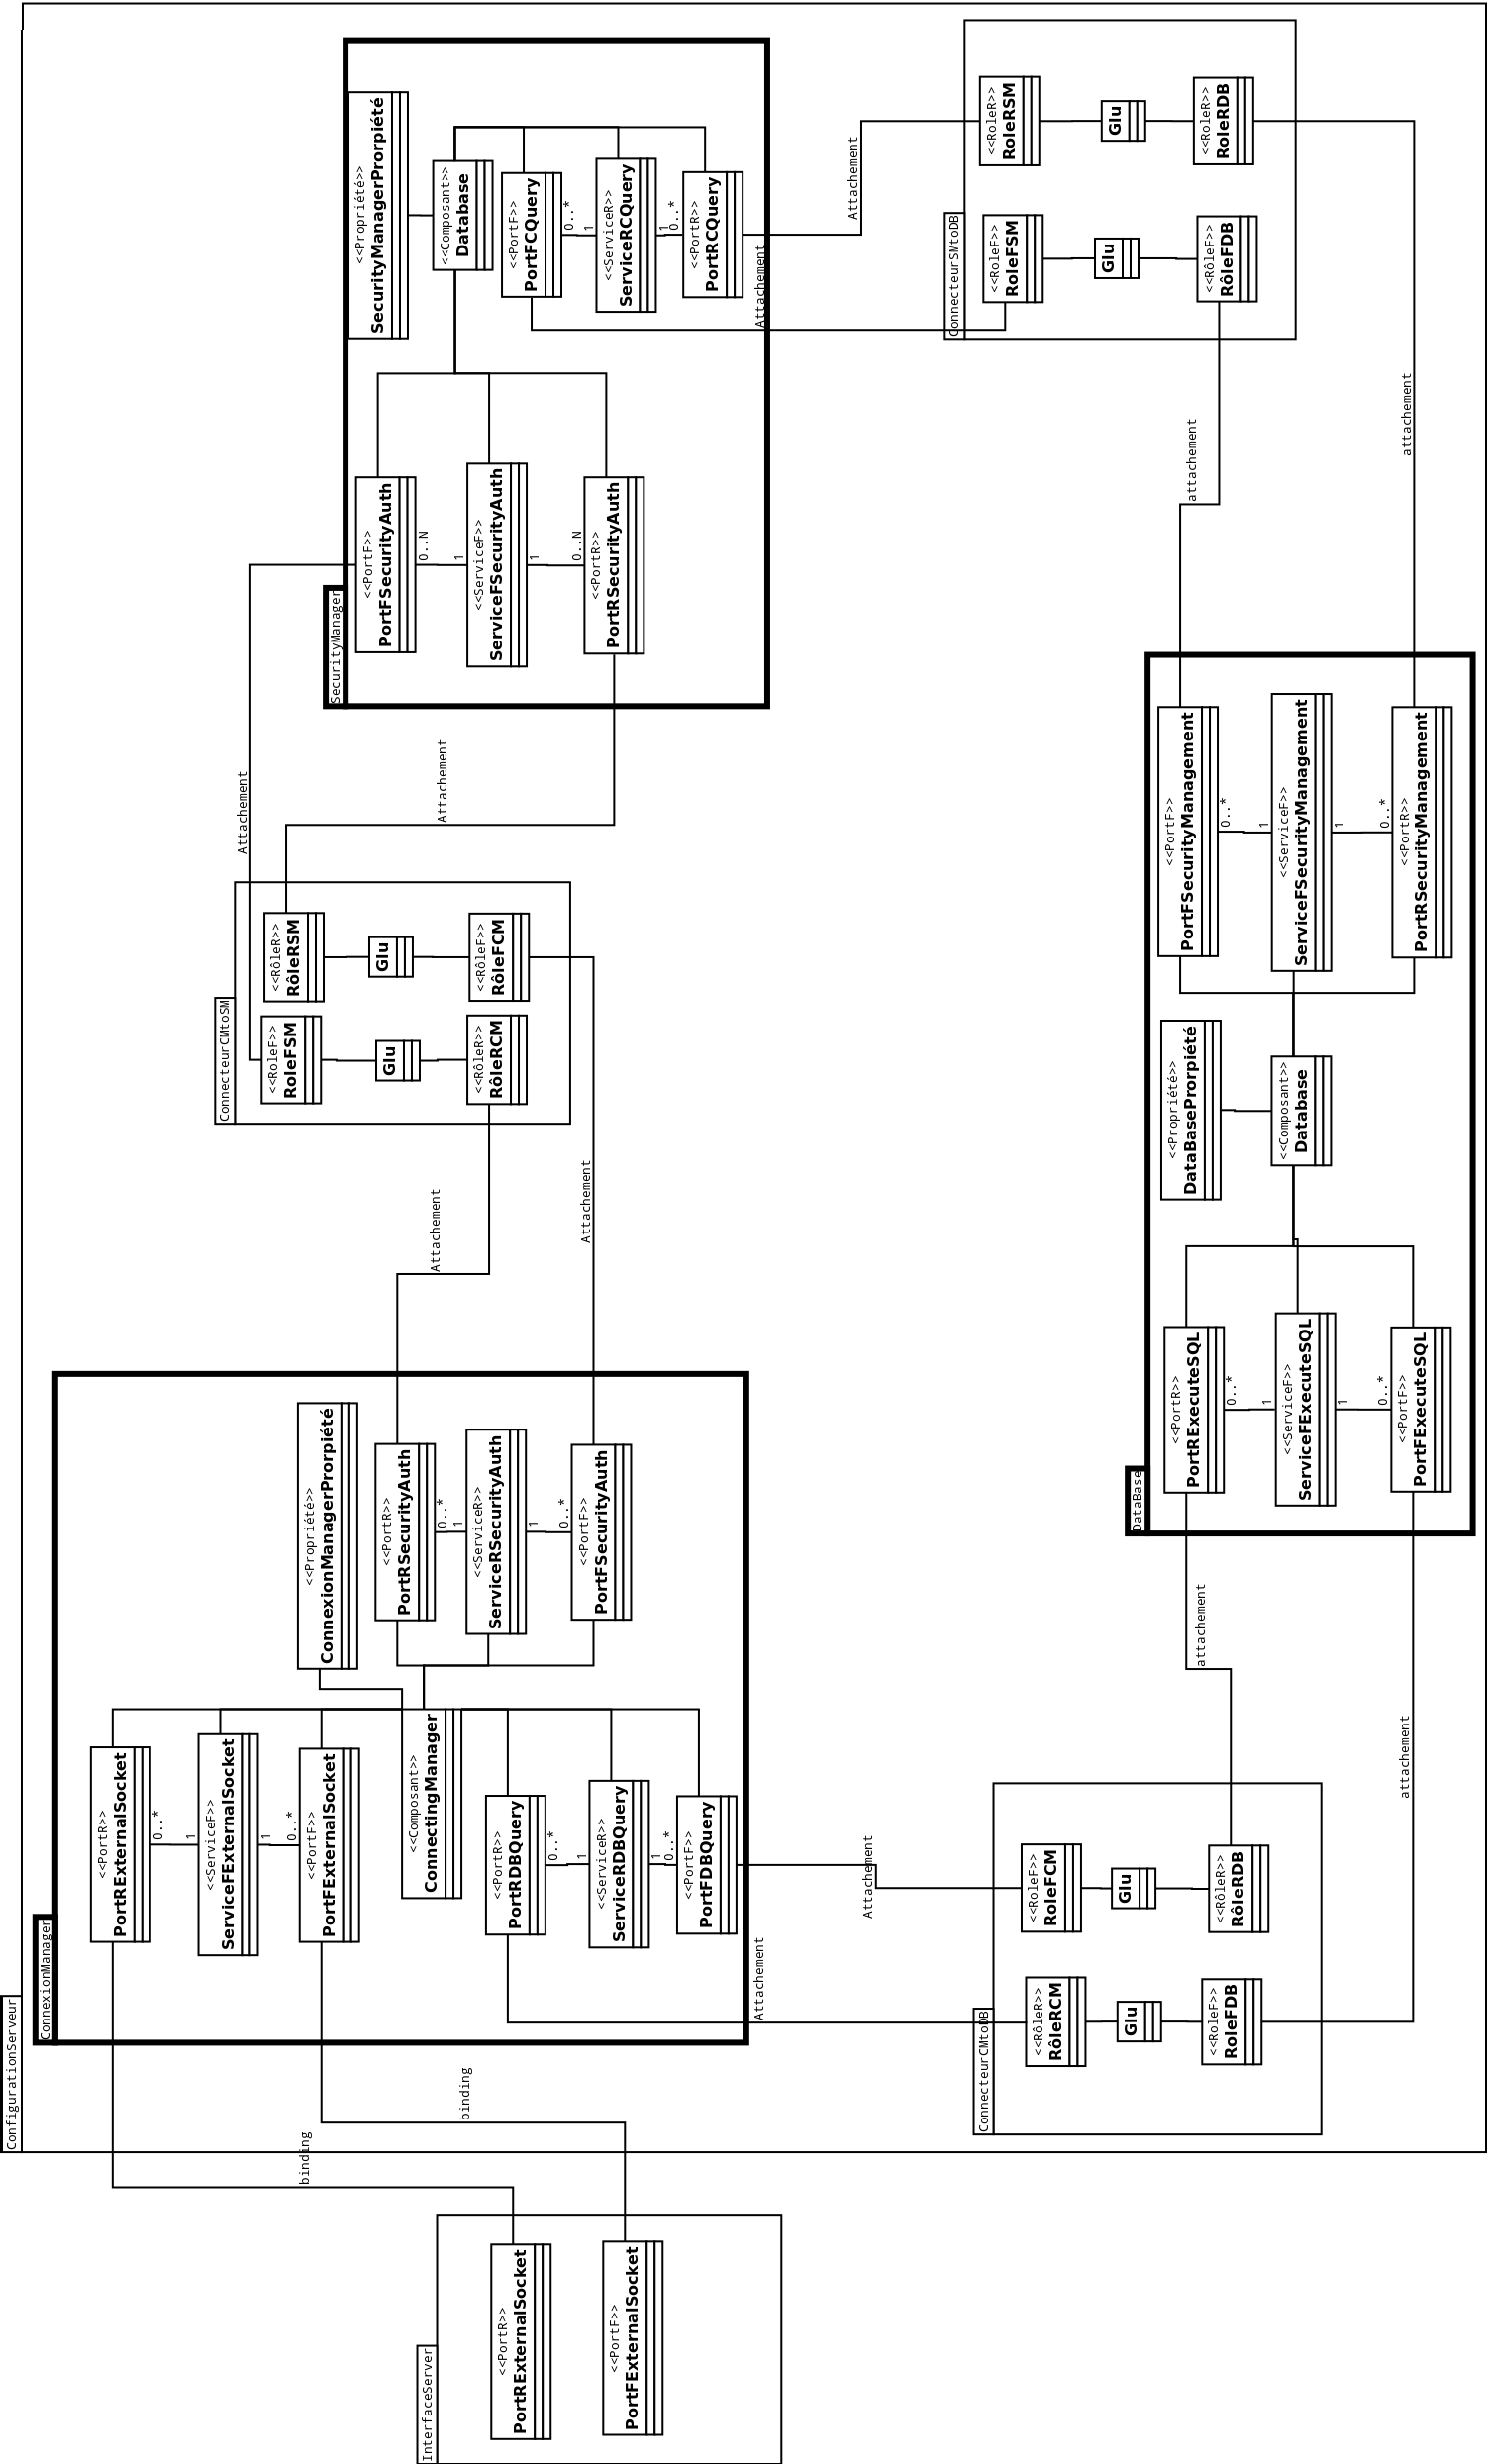
\includegraphics[scale=0.20]{img/M1}
  \caption{Model (M1)}
  \label{fig:M1}
\end{figure}
